%%%%%%%%%%%%%%%%%%%%%%%%%%%%%%%%%%%%%%%%%%%%%%%%%%%%%%%%%%%%%%%%%%%%%%%%%%%%%%%%
%2345678901234567890123456789012345678901234567890123456789012345678901234567890
%        1         2         3         4         5         6         7         8

%\documentclass[letterpaper, 10 pt, conference]{ieeeconf}  % Comment this line out if you need a4paper

\documentclass[a4paper, 10pt, conference]{ieeeconf}      % Use this line for a4 paper

\IEEEoverridecommandlockouts                              % This command is only needed if 
                                                          % you want to use the \thanks command

\overrideIEEEmargins                                      % Needed to meet printer requirements.

% See the \addtolength command later in the file to balance the column lengths
% on the last page of the document

% The following packages can be found on http:\\www.ctan.org
%\usepackage{graphics} % for pdf, bitmapped graphics files
%\usepackage{epsfig} % for postscript graphics files
%\usepackage{mathptmx} % assumes new font selection scheme installed
%\usepackage{times} % assumes new font selection scheme installed
%\usepackage{amsmath} % assumes amsmath package installed
%\usepackage{amssymb}  % assumes amsmath package installed
\usepackage{graphicx}
\usepackage[export]{adjustbox}
\graphicspath{ {images/} }


\title{\LARGE \bf
Collaboration between Multiple Automouns Cars
}

\author{Kathy Lu$^{1}$, Simon Hsieh$^{2}$ and Ding-Hao Lin$^{3}$% <-this % stops a space
\thanks{* This work was supported by the Robotics Master Program in National Chiao Tung University, Taiwan}% <-this % stops a space
\thanks{$^{1}$Kathy Lu, National Chiao Tung University, Taiwan.
        {\tt\small kathylu0424@gmail.com}}%
\thanks{$^{2}$Simon Hsieh, National Chiao Tung University, Taiwan.
        {\tt\small simon10030950@gmail.com}}%
\thanks{$^{3}$Ding-Hao Lin, National Chiao Tung University, Taiwan.
        {\tt\small wx9341313@gmail.com}}%
}


\begin{document}



\maketitle
\thispagestyle{empty}
\pagestyle{empty}

%%%%%%%%%%%%%%%%%%%%%%%%%%%%%%%%%%%%%%%%%%%%%%%%%%
\section{INTRODUCTION \& MOTIVATION}

Since we are entering the generation of industry 4.0, many factories are starting to change to automount way for logistics work. More and more factories are using automatic guided vehicle (AGV) system to help them transport objects from place to place. Moreover, AGV system is very efficient and cost-reducing.

Like factory, other places such as school, hospital and company also have same requirements for logistics. Workers in this place spend lots of time to exchange documents, deliver medical supplies and other stuffs. We expect that workers can save lots of time and effort in logistics work and focus more on their jobs if we implement AGV system in these places. 

However, current AGV system is designed for factory, which means they have huge size and could only navigate through limited routes which have less people walking around. Therefore it is not suitable for school, hospital and company which are complicated with lots of obstacles and human. 

To solve this problem, our team aims to develop a small AGV system which can be used in school or hospital to deliver stuffs. We design a small size autonomous car which can navigate through places to target location, avoid obstacles and human, recognize and grasp specific object, and communicate with other autonomous cars.

\begin{figure}[t]
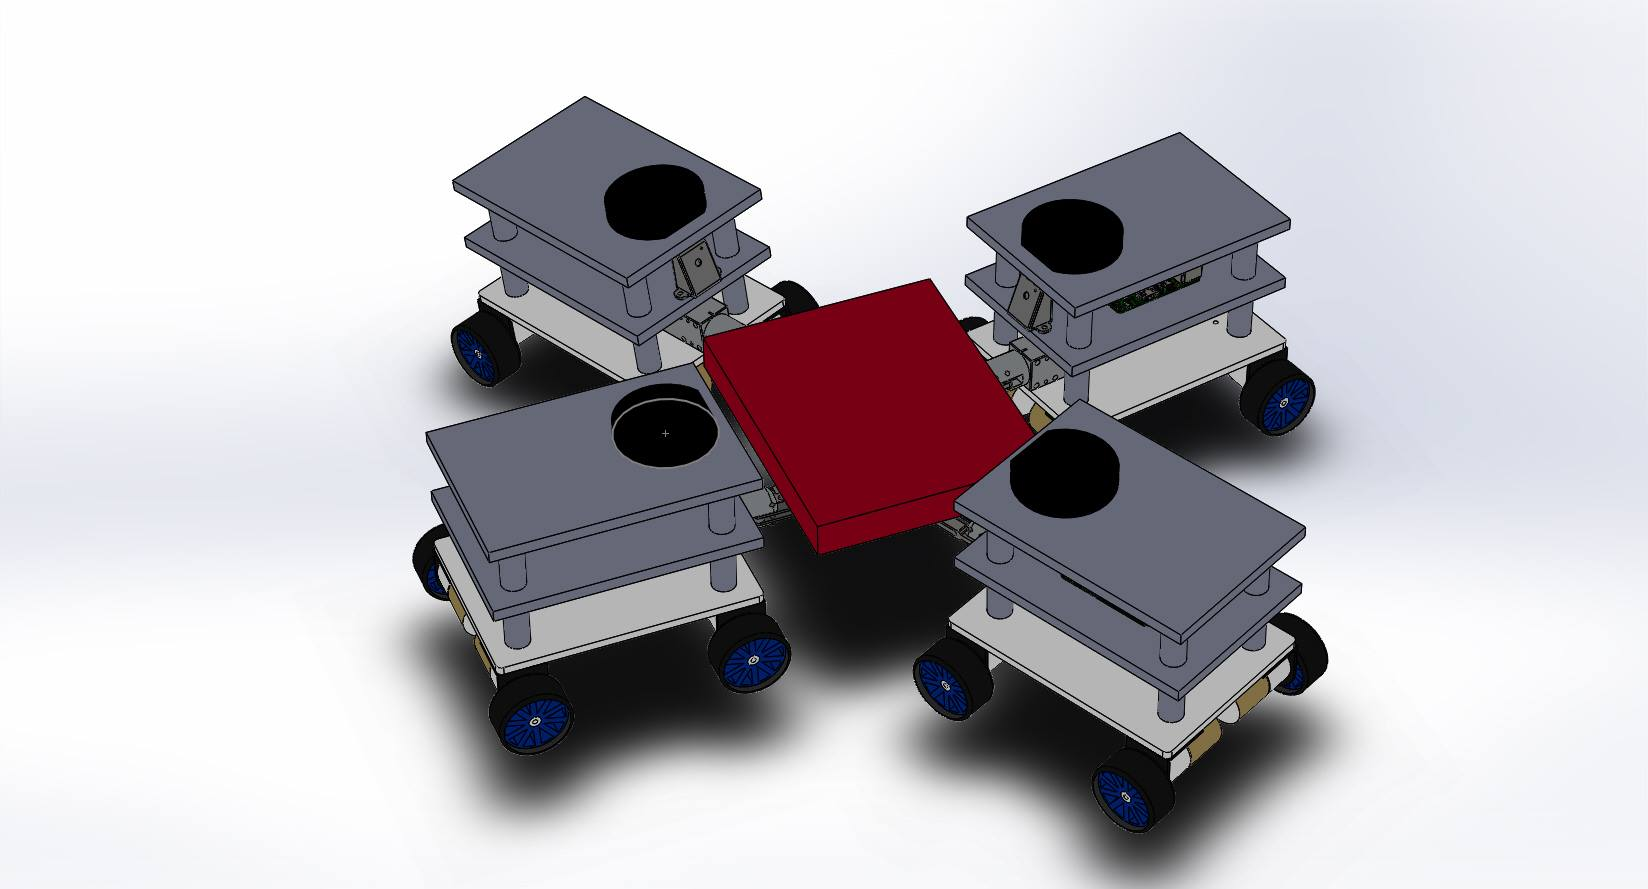
\includegraphics[width=0.95\columnwidth]{Teaser}
\centering
\caption{We will first build one autonomous car. Our car can navigate through places and recognize objects. Next, we will build another two to three cars based on our first edition. At last, by exchanging information with others, our robots can be able to do some collaboration. For example in this figure, we aim to grasp a bigger object with collaboration between four cars.}
\end{figure}

%%%%%%%%%%%%%%%%%%%%%%%%%%%%%%%%%%%%%%%%%%%%%%%%%%%
\section{SYSTEM ARCHITECTURE \& EQUIPMENTS}
\subsection{SYSTEM ARCHITECTURE}

\begin{figure}[h]
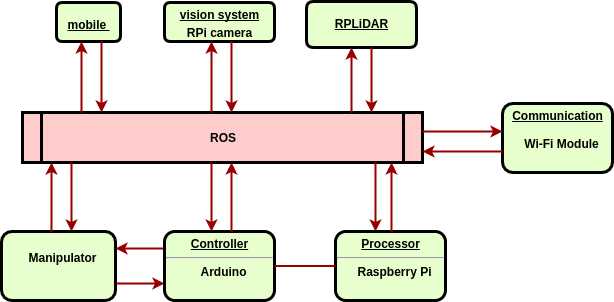
\includegraphics[width=0.95\columnwidth]{system_architecture}
\centering
\caption{System architecture for automouns car system.}
\end{figure}

We will build a mobile platform with microprocessor, controller, other sensors and manipulator. The gripper of manipulator should be stable enough to grasp reasonable weight. 

Microprocessor is the main part of the system, consider the price and ability, we use Raspberry Pi 3 Model B+ which install ROS on it as middleware to accept signals from other hardware such motor and sensors and give them command. Also we use Arduino UNO as controller to accept the command from Raspberry pi to control motors.

RPLiDAR is used to detect surrounding environment and send information to ROS for SLAM. RPi camera is used to capture the image which contain AprilTag and send back to ROS.

When autonomous cars are trying to collaborate, Wi-Fi Module is used to exchange data with others to get location or other information. One of  autonomous cars will collects all data, estimate the pose and send the pose information to other autonomous cars.



%%%%%%%%%%%%%%%%%%%%%%%%%%%%%%%%%%%%%%
\subsection{EQUIPMENTS} 

\begin{itemize}
\item Mobile

\begin{itemize}
	\item Micro-processor: Raspberry Pi 3 model B+
	\item Controller: Arduino
	\item GM25-370 DC Motors with encoder
	\item Mobile chassis strucure
	\item battery
\end{itemize}

\item Manipulator
\begin{itemize}
	\item AX12-A Motors
	\item Gripper
\end{itemize}

\item Sensors
\begin{itemize}
	\item Rpi-camera
	\item RPLiDar
	\item Router
\end{itemize}

\end{itemize}

\begin{figure}[h]
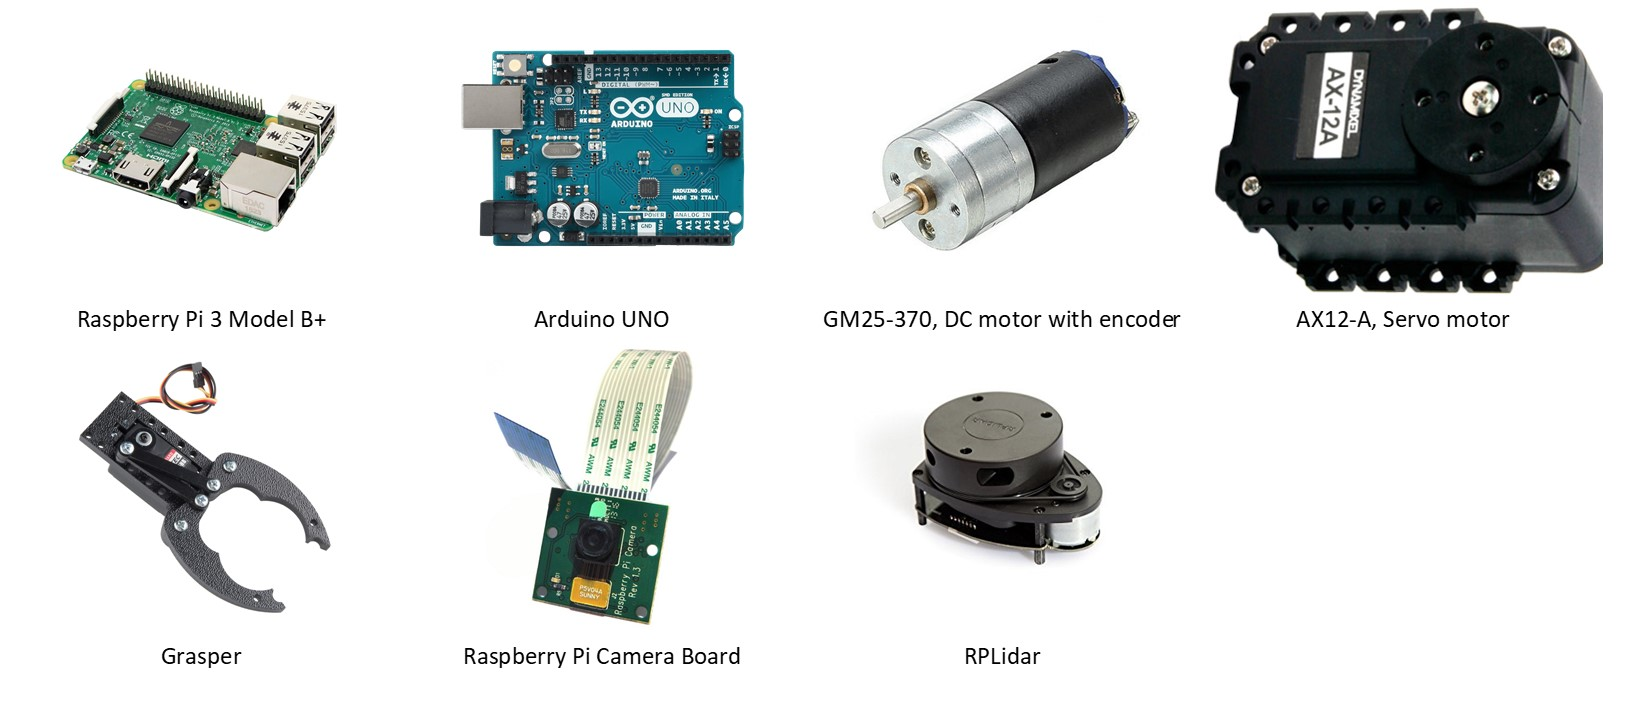
\includegraphics[width=0.95\columnwidth]{equipment}
\centering
\caption{Some equipments are used in the project.}
\end{figure}

%%%%%%%%%%%%%%%%%%%%%%%%%%%%%%%%%%%%%%%%%%%%%%
%%%%%%%%%%%%%%%%%%%%%%%%%%%%%%%%%%%%%%%%%%%%%%
\section{SPECIFIC AIMS}
\begin{itemize}
\item Mobile
\begin{itemize}
	\item Construct a stable structure for autonomous car.
	\item SLAM for localization with the help of RPLiDAR.
	\item Obstacle avoidance.
	\item Be able to move from the specific location to target location using RRT.
\end{itemize}

\item Recognizing apriltag
\begin{itemize}
    \item Recognize the specific object (with apriltag) and show it on map (RGB-D Camera)
\end{itemize}

\item Manipulator
\begin{itemize}
	\item Stable Structure
	\item Grasping
	\item Be able to put the specific object to a specific location (AprilTag)
\end{itemize}

\item Collaboration
\begin{itemize}
	\item Communication with each other
	\item Knowing others’ locations
	\item Grasp the specific object together
	\item Multiple cars move to multiple destinations respectively
\end{itemize}
\end{itemize}

%%%%%%%%%%%%%%%%%%%%%%%%%%%%%%%%%%
\section{APPROACH}

\subsection{Mobile}
\begin{itemize}
\item Structure
\begin{itemize}
	\item Consider the center gravity and other equipments on the mobile, design a stable structure and assemble them.
	\item Test which kind of structure is more suitable for our system, 2 or 3 layers.
\end{itemize}

\item Mobile
\begin{itemize}
	\item Install Ubuntu 14.04 or 16.04 and ROS on Raspberry Pi.
	\item Use SSH connect to computer.
	\item Simulate it on the Rviz.
\end{itemize}

\item SLAM
\begin{itemize}
	\item Create a 2D map by navigating autonomous car with teleoperation.
	\item Try both Gmapping SLAM and Hector SLAM on our robot and check which one is more effective.
\end{itemize}

\item Route Planning
\begin{itemize}
	\item Use RRT algorithm to do the navigation.
	\item Avoid still obstacles.
	\item Avoid dynamic obstacles.
\end{itemize}
\end{itemize}

\subsection{Recognizing apriltag}
\begin{itemize}
\item Use raspberry-pi cemera(or other RGB-D cemera) to capture the real-time image.
\item Use openCV to recognize AprilTag.
\item Use TF and Pin hole projection to calculate the distance between the AprilTag and robot's location.
\item Add the location of AprilTag on the map.
\end{itemize}

\subsection{Manipulator}
\begin{itemize}
	\item Make a stable structure. Use Solidwork to draw the structure of gripper.
	\item Use 3D printer to build our gripper.
	\item Install a gripper in AX12A motor.
	\item Equip it on our autonomous car.
	\item Calculate the distance between AprilTag and object then grasp it.
\end{itemize}



\subsection{Collaboration}
\begin{itemize}
	\item Two autonomous cars can exchange messages through Wi-Fi.
	\item Two or more autonomous cars can submit their location information through Wi-Fi.
	\item Add other autonomous cars’ location on the map.See Figure. 4.
	\item Calculate and exchange the distance information between cars and AprilTags. Decide a most efficient plan for all the autonomous cars in the team.
	\item Estimate other’s pose and grasp an object and ove to the destination together.
\end{itemize}

\begin{figure}[h]
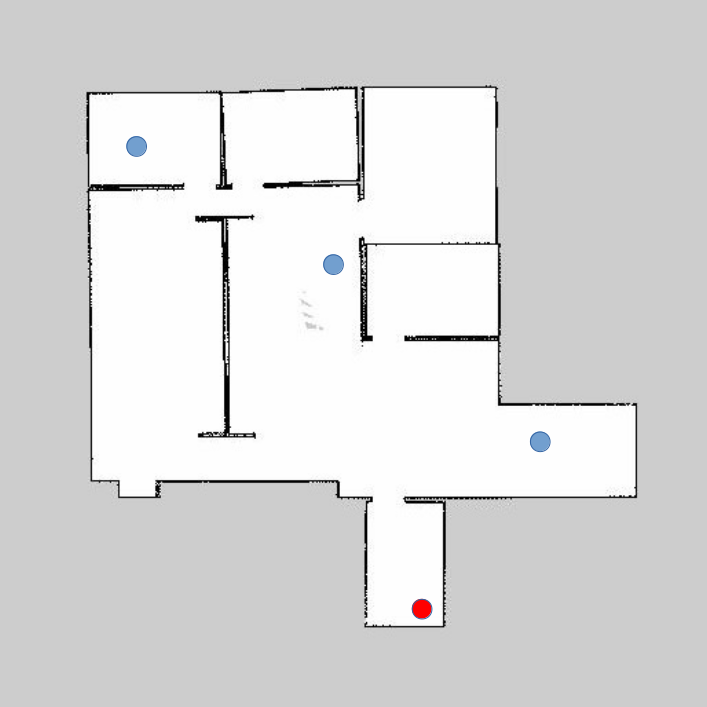
\includegraphics[width=0.95\columnwidth]{collaboration}
\centering
\caption{The map after 4 autonomous cars exchage thier location information and add on the map.}
\end{figure}


%%%%%%%%%%%%%%%%%%%%%%%%%%%%%%%%%%%%%%%%%%%%%%%%%%%%%%%%
\section{SCHEDULE AND TEAM COLLABORATION}
The estimated timeline of the project, our team divides project into 4 parts. We will start from  week 10 and finish on week 17.
\begin{figure}[h]
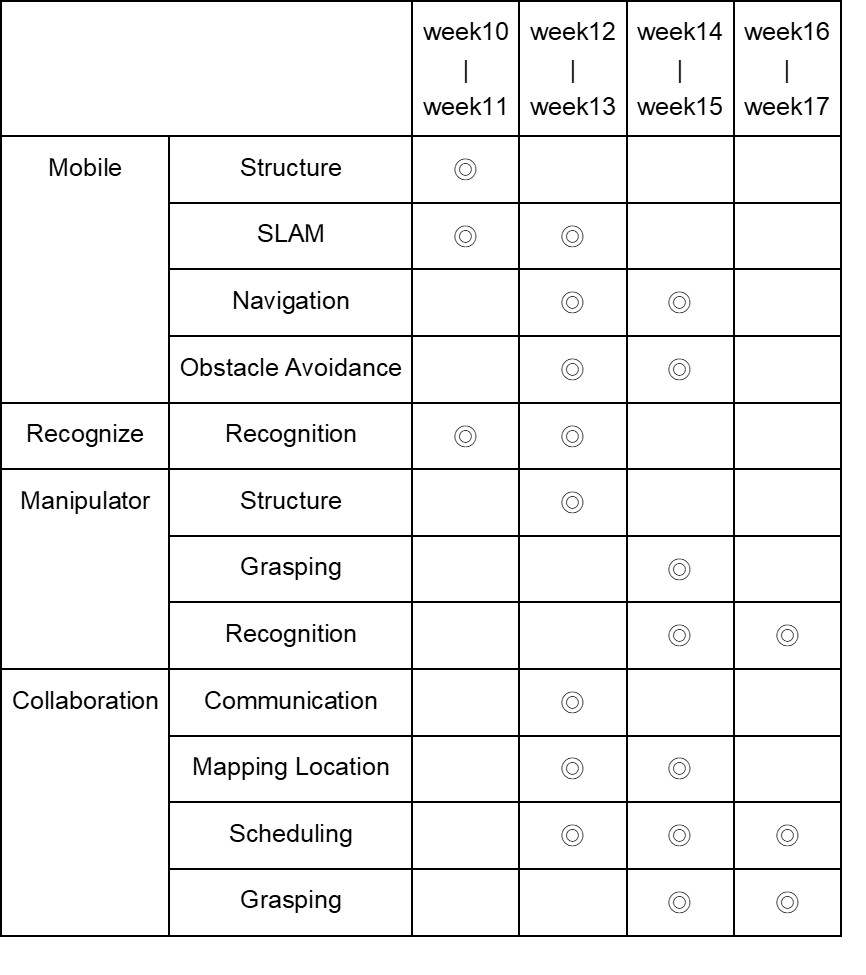
\includegraphics[width=0.95\columnwidth]{schedule}
\centering
\end{figure}

\addtolength{\textheight}{-12cm}   % This command serves to balance the column lengths
                                  % on the last page of the document manually. It shortens
                                  % the textheight of the last page by a suitable amount.
                                  % This command does not take effect until the next page
                                  % so it should come on the page before the last. Make
                                  % sure that you do not shorten the textheight too much.


\end{document}
